% Feature Model of the tsam aggregation configuration.
%
% Notation: FODA feature diagram (Kang et al., Feature-Oriented Domain
% Analysis, CMU/SEI-90-TR-21, 1990), as used in the software-product-line
% literature and by FeatureIDE:
%   filled circle on an edge   = MANDATORY feature
%   open circle on an edge     = OPTIONAL feature
%   unfilled arc across a fan  = ALTERNATIVE group (choose EXACTLY ONE)
%   filled arc across a fan    = OR group (choose ONE OR MORE)
%   dashed arrow               = cross-tree constraint (requires)
%
% ── WHAT CHANGED IN THIS REVISION, AND WHY ────────────────────────────────
%  1. COLUMNS ARE IN PIPELINE PHASE ORDER: Weighting (Phase 1), Grouping and
%     Representation (Phase 2), then Extreme periods, Rescaling and
%     Segmentation (Phase 3). The previous revision led with the two mandatory
%     groups, which read as importance order and did not line up with Fig. 1.
%  2. THE ARCS SPAN EVERY EDGE OF THEIR GROUP, not just the first two. That is
%     what FODA actually prescribes, and it is also the fix for their being
%     hard to see: the Grouping arc is now 50 mm tall rather than a 10 mm lens
%     tucked against the bus. The bus also moved from ci-14 to ci-15, so a 3 mm
%     arc bulge clears it by 1.5 mm instead of touching it.
%  3. THE DISTRIBUTION PARAMETERS ARE DRAWN. `distribution` is not a leaf: it
%     is the Distribution dataclass (config.py:55-114) with scope,
%     preserve_minmax and five concurrency strategies. Those are the options
%     that existed nowhere in the figure set. They need a third tree level,
%     which does not fit a 27 mm column, so they get their own band with 53 mm
%     columns — where the arcs are unmistakable.
%  4. BOTH TEXT BLOCKS ARE GONE. The "why two mandatory groups" callout and the
%     written cross-tree constraint are caption material; the figure carries
%     only the drawing and the legend.
%  5. THE DEPRECATED REPRESENTATION STRINGS ARE GONE. `distribution_minmax` is
%     exactly Distribution(preserve_minmax=True), which band 2 already shows,
%     and `minmax_mean` as a bare string silently returns plain mean because
%     nothing can carry the column lists through it. Representation therefore
%     offers five alternatives, with the two parameterized ones named as the
%     classes they are: Distribution and MinMaxMean.
%
% ── WHAT MOVED TO THE CAPTION ─────────────────────────────────────────────
% The kmedoids -> MILP solver constraint is no longer in the figure. It cannot
% be drawn: the kmedoids leaf is boxed in by the Representation column's bus on
% one side and its own column's leaves below, with no clear lane to any free
% space. It belongs in the caption, together with the note that
% `distribution_minmax` is shorthand for `preserve_minmax=True` and
% `reference_attribute` for `concurrency="reference"`.
%
% ── PRINT TARGET ──────────────────────────────────────────────────────────
% Same budget as the rest of the set: text column 165.1 x 228.6 mm, figures
% placed at full width, so ASPECT h/w <= 1.24 and WIDTH <= ~165 mm.
% This file is ~164 x ~201 mm, aspect ~1.23 — just inside, which is why the
% band-2 pitches below are 9 mm rather than 10 mm. If anything is added, the
% aspect is what will break first, so re-measure.
%
% ── LAYOUT GRID (millimetres, y negative downwards) ───────────────────────
% BAND 1 — six columns, pitch 27, boxes 24.5 mm wide:
%   c1 = 17 Weighting   c2 = 44 Grouping     c3 = 71 Representation
%   c4 = 98 Extremes    c5 = 125 Rescaling   c6 = 152 Segmentation
%   root (84.5,-8) 44x9   bar y -18   markers y -20.7   groups y -24..-35
%   leaf bus x = ci-15, elbow y -38, stub ci-15 -> ci-10.5
%   leaves 21 mm wide (ci +/- 10.5), rows -46 -56 -66 -76 -86 -96
%   arcs: x radius 3 at (ci-10.5, first row), y radius = half the row span
% CONNECTOR to band 2: (81.5,-76) -- (86,-76) -- (86,-107). x = 86 clears c4's
%   leaves (87.5..108.5) and c4's bus (x 83, y -38..-68 — disjoint in y).
% BAND 2 — three columns, pitch 53, boxes 44 mm wide:
%   c1 = 30 scope   c2 = 83 concurrency   c3 = 136 preserve_minmax
%   root (84.5,-112) 44x10   bar y -124   markers y -126.5
%   groups y -129.5..-140.5   leaf bus x = ci-27, elbow y -144
%   leaves 40 mm wide (ci +/- 20), rows -151 -160 -169 -178 -187 (pitch 9)
%   arcs: x radius 4 at (ci-20, -151); bus clearance 3 mm
%   constraint lane x = 53.5: clears c1's group (ends 52) by 1.5 mm and c2's
%     bus (56) by 2.5 mm, and passes c1's and c2's elbows at y -144 outside
%     both their x-ranges.
% Band 2 puts concurrency in c2 SO THAT the constraint edge is short: it runs
% from concurrency's west edge to the `local` leaf in c1. With concurrency in
% c3 every route crossed either c2's group box or c3's bus.
%
% ── TRAPS RE-CHECKED HERE (see the project notes) ─────────────────────────
%   * A TikZ node CLIPS NOTHING and LaTeX will not break a line at `\_`, so
%     every long snake_case leaf is broken by hand. `rescale_exclude_columns`
%     is 23 characters — 39 mm at \scriptsize, far past its 21 mm box — so it
%     is the one leaf set in \tiny.
%   * `minimum height` is a MINIMUM: a three-line leaf grows its own box, so
%     the row pitch, not the box height, is what has to leave the gap.
%   * A TikZ STYLE cannot be applied to part of a node's text; the phase tags
%     use a \newcommand DECLARATION.
%   * Guillemets via \guillemotleft/\guillemotright, \textperiodcentered{}, ---.
%
% Regenerate:
%   tectonic feature_model.tex
%   pdftocairo -svg feature_model.pdf feature_model.svg

\documentclass[10pt,border=1mm]{standalone}
\usepackage[T1]{fontenc}
\usepackage{lmodern}
\usepackage{tikz}
\usetikzlibrary{positioning,arrows.meta,fit,backgrounds,calc}

\definecolor{fzjblue}{HTML}{023D6B}
\definecolor{fzjdark}{HTML}{012845}
\definecolor{tintblue}{HTML}{DCE9F2}
\definecolor{amber}{HTML}{A8681A}
\definecolor{ambertint}{HTML}{FBF1E4}
\definecolor{greytext}{HTML}{3F4A55}

% A DECLARATION, not a TikZ style: a style cannot be applied to part of a
% node's text, which is what the phase tags need.
\newcommand{\ph}{\tiny\color{greytext}}

\begin{document}
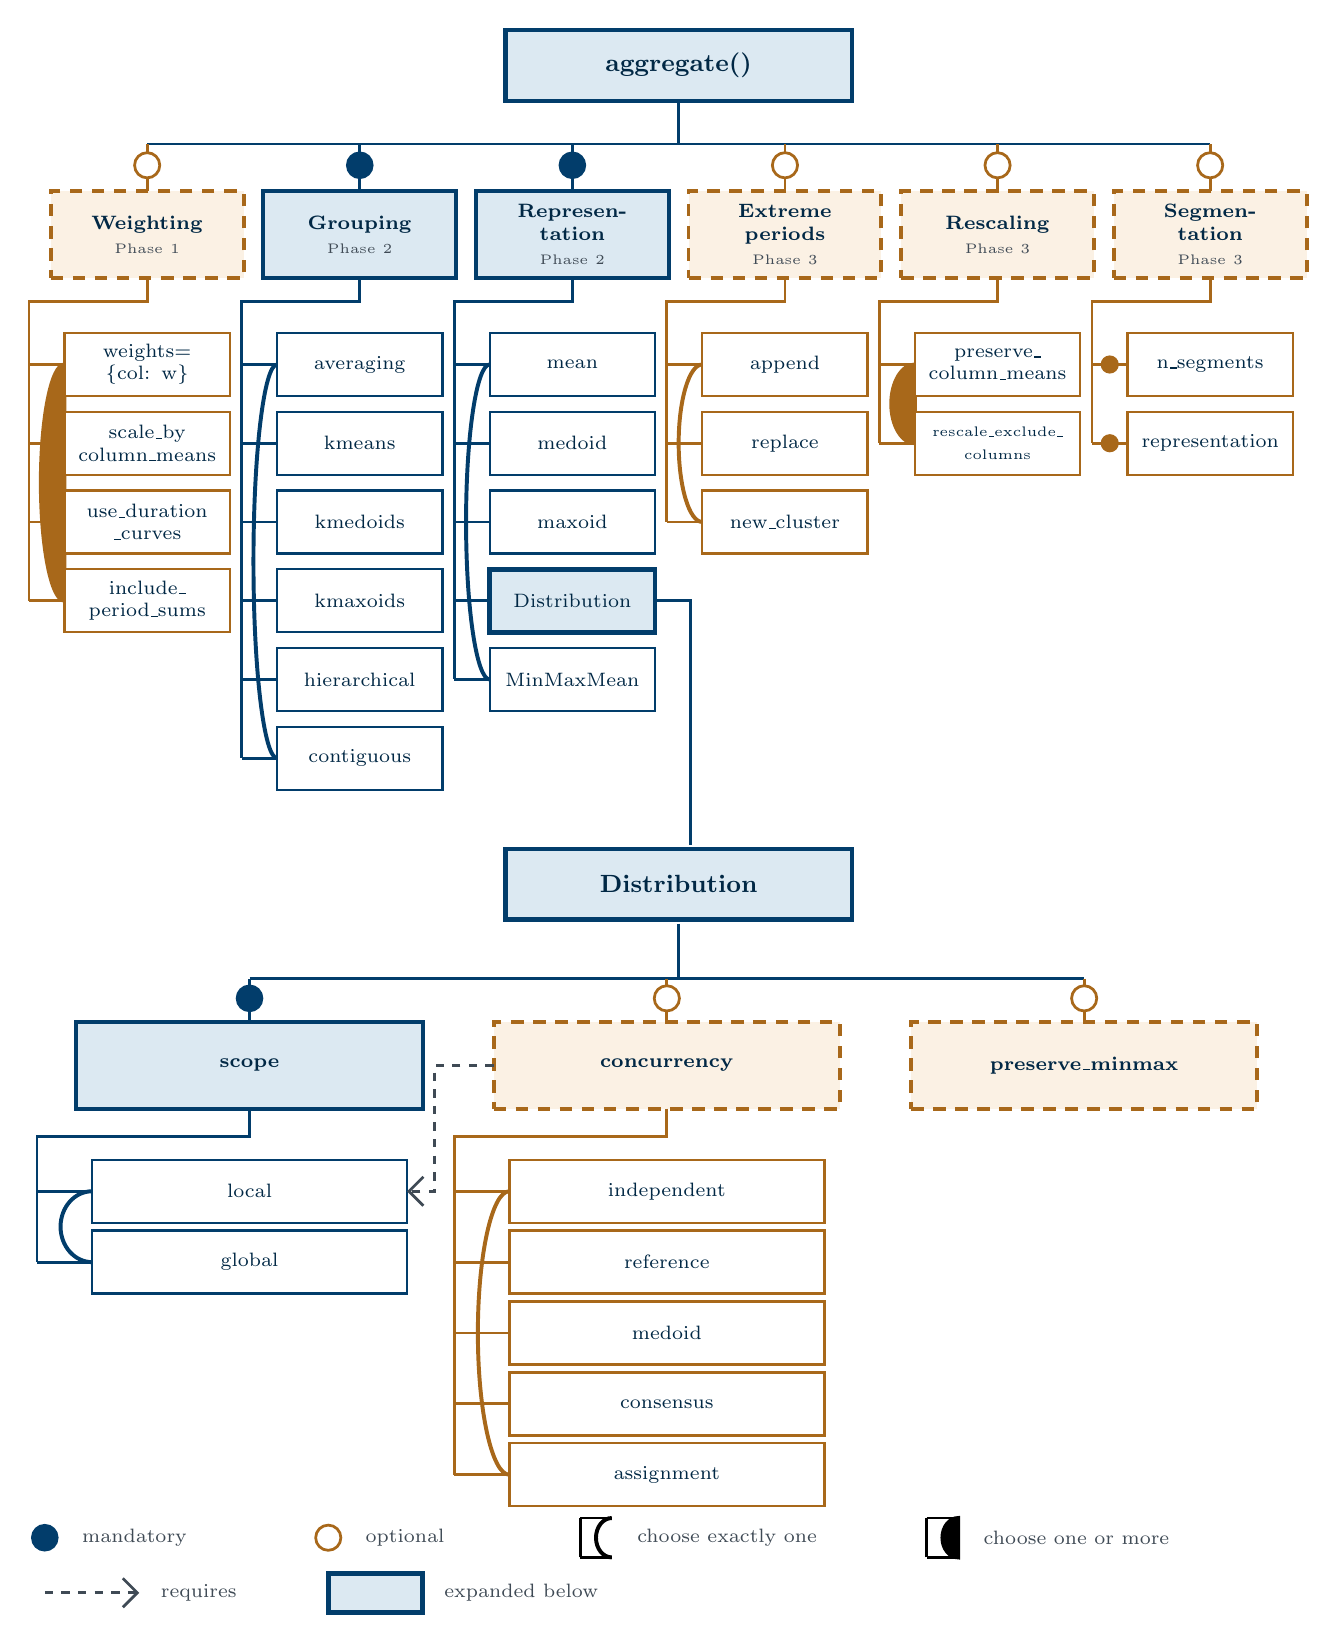
\begin{tikzpicture}[
  x=1mm, y=1mm,
  root/.style={
    draw=fzjblue, line width=0.55mm, fill=tintblue, text=fzjdark,
    minimum width=44mm, minimum height=9mm, text width=40mm,
    align=center, font=\small\bfseries},
  grpm/.style={
    draw=fzjblue, line width=0.5mm, fill=tintblue, text=fzjdark,
    minimum width=24.5mm, minimum height=11mm, text width=21.5mm,
    align=center, font=\scriptsize},
  grpo/.style={
    draw=amber, line width=0.5mm, dash pattern=on 1.6mm off 1.2mm,
    fill=ambertint, text=fzjdark,
    minimum width=24.5mm, minimum height=11mm, text width=21.5mm,
    align=center, font=\scriptsize},
  leaf/.style={
    draw=fzjblue, line width=0.3mm, fill=white, text=fzjdark,
    minimum width=21mm, minimum height=8mm, text width=18.5mm,
    align=center, font=\scriptsize},
  leafo/.style={
    draw=amber, line width=0.3mm, fill=white, text=fzjdark,
    minimum width=21mm, minimum height=8mm, text width=18.5mm,
    align=center, font=\scriptsize},
  % the one leaf that is expanded in band 2
  leafx/.style={leaf, line width=0.6mm, fill=tintblue},
  % band 2
  grp2m/.style={grpm, minimum width=44mm, text width=41mm},
  grp2o/.style={grpo, minimum width=44mm, text width=41mm},
  leaf2/.style={leaf, minimum width=40mm, text width=37.5mm},
  leaf2o/.style={leafo, minimum width=40mm, text width=37.5mm},
  edge/.style={draw=fzjblue, line width=0.35mm},
  edgeo/.style={draw=amber, line width=0.35mm},
  % In the DRAWING the arcs keep their column's colour, so a group reads as
  % mandatory or optional at a glance. In the LEGEND they are black (arck /
  % edgek below): the two group kinds are colour-independent — "choose one or
  % more" applies equally to a blue mandatory group and an amber optional one —
  % and drawing the key glyph in one of those two colours implied otherwise.
  arc/.style={draw=fzjblue, line width=0.5mm},
  arco/.style={draw=amber, line width=0.5mm},
  arck/.style={draw=black, line width=0.5mm},
  edgek/.style={draw=black, line width=0.35mm},
  req/.style={-{Straight Barb[scale=1.5]}, dashed, draw=greytext,
              line width=0.35mm},
  lgd/.style={font=\scriptsize, text=greytext, anchor=west}
]
\hyphenpenalty=10000 \exhyphenpenalty=10000

% ══════════════════════════════════════════════════════════════════════════
% BAND 1 — the six top-level groups, in pipeline phase order
% ══════════════════════════════════════════════════════════════════════════
\node[root] (root) at (84.5,-8) {aggregate()};
\draw[edge] (84.5,-12.5) -- (84.5,-18);
\draw[edge] (17,-18) -- (152,-18);

% mandatory (filled marker): Grouping, Representation
\foreach \x in {44,71}{
  \draw[edge] (\x,-18) -- (\x,-24);
  \node[circle, draw=fzjblue, fill=fzjblue, line width=0.3mm,
        minimum size=3.2mm, inner sep=0] at (\x,-20.7) {};
}
% optional (open marker): Weighting, Extremes, Rescaling, Segmentation
\foreach \x in {17,98,125,152}{
  \draw[edgeo] (\x,-18) -- (\x,-24);
  \node[circle, draw=amber, fill=white, line width=0.35mm,
        minimum size=3.2mm, inner sep=0] at (\x,-20.7) {};
}

\node[grpo] at ( 17,-29.5) {\textbf{Weighting}\\[0.3mm]{\ph Phase 1}};
\node[grpm] at ( 44,-29.5) {\textbf{Grouping}\\[0.3mm]{\ph Phase 2}};
\node[grpm] at ( 71,-29.5) {\textbf{Represen-}\\\textbf{tation}\\[0.3mm]{\ph Phase 2}};
\node[grpo] at ( 98,-29.5) {\textbf{Extreme}\\\textbf{periods}\\[0.3mm]{\ph Phase 3}};
\node[grpo] at (125,-29.5) {\textbf{Rescaling}\\[0.3mm]{\ph Phase 3}};
\node[grpo] at (152,-29.5) {\textbf{Segmen-}\\\textbf{tation}\\[0.3mm]{\ph Phase 3}};

% ── c1 Weighting — OR group (filled arc), 4 leaves ────────────────────────
\draw[edgeo] (17,-35) -- (17,-38) -- (2,-38) -- (2,-76);
\foreach \y in {-46,-56,-66,-76}{ \draw[edgeo] (2,\y) -- (6.5,\y); }
\filldraw[arco, fill=amber]
  (6.5,-46) arc[start angle=90, end angle=270, x radius=3mm, y radius=15mm] -- cycle;
\node[leafo] at (17,-46) {weights=\\\{col: w\}};
\node[leafo] at (17,-56) {scale\_by\\column\_means};
\node[leafo] at (17,-66) {use\_duration\\\_curves};
\node[leafo] at (17,-76) {include\_\\period\_sums};

% ── c2 Grouping — ALTERNATIVE group (unfilled arc), 6 leaves ──────────────
\draw[edge] (44,-35) -- (44,-38) -- (29,-38) -- (29,-96);
\foreach \y in {-46,-56,-66,-76,-86,-96}{ \draw[edge] (29,\y) -- (33.5,\y); }
\draw[arc] (33.5,-46) arc[start angle=90, end angle=270, x radius=3mm, y radius=25mm];
\node[leaf] at (44,-46) {averaging};
\node[leaf] at (44,-56) {kmeans};
\node[leaf] at (44,-66) {kmedoids};
\node[leaf] at (44,-76) {kmaxoids};
\node[leaf] at (44,-86) {hierarchical};
\node[leaf] at (44,-96) {contiguous};

% ── c3 Representation — ALTERNATIVE group, 6 leaves ───────────────────────
% `distribution` is drawn heavier and tinted: it is the one leaf that carries a
% sub-tree, expanded in band 2.
% Five leaves, not six. The `distribution_minmax` and `minmax_mean` STRINGS are
% proposed for deprecation and are gone: the first is exactly
% Distribution(preserve_minmax=True), which band 2 already carries, and the
% second silently returns plain mean because a bare string cannot carry the
% column lists. What survives is the two objects, named as the classes they
% are. MinMaxMean is deliberately NOT expanded: its max_columns / min_columns
% are lists of column names — data, not variability — and a feature model
% models the latter. `reference_attribute` is omitted for the same reason.
\draw[edge] (71,-35) -- (71,-38) -- (56,-38) -- (56,-86);
\foreach \y in {-46,-56,-66,-76,-86}{ \draw[edge] (56,\y) -- (60.5,\y); }
\draw[arc] (60.5,-46) arc[start angle=90, end angle=270, x radius=3mm, y radius=20mm];
\node[leaf]  at (71,-46) {mean};
\node[leaf]  at (71,-56) {medoid};
\node[leaf]  at (71,-66) {maxoid};
\node[leafx] at (71,-76) {Distribution};
\node[leaf]  at (71,-86) {MinMaxMean};

% ── c4 Extreme periods — ALTERNATIVE group, 3 leaves ──────────────────────
\draw[edgeo] (98,-35) -- (98,-38) -- (83,-38) -- (83,-66);
\foreach \y in {-46,-56,-66}{ \draw[edgeo] (83,\y) -- (87.5,\y); }
\draw[arco] (87.5,-46) arc[start angle=90, end angle=270, x radius=3mm, y radius=10mm];
\node[leafo] at (98,-46) {append};
\node[leafo] at (98,-56) {replace};
\node[leafo] at (98,-66) {new\_cluster};

% ── c5 Rescaling — OR group, 2 leaves ─────────────────────────────────────
\draw[edgeo] (125,-35) -- (125,-38) -- (110,-38) -- (110,-56);
\foreach \y in {-46,-56}{ \draw[edgeo] (110,\y) -- (114.5,\y); }
\filldraw[arco, fill=amber]
  (114.5,-46) arc[start angle=90, end angle=270, x radius=3mm, y radius=5mm] -- cycle;
\node[leafo] at (125,-46) {preserve\_\\column\_means};
\node[leafo] at (125,-56) {\tiny rescale\_exclude\_\\columns};

% ── c6 Segmentation — no group arc: both children are mandatory once on ───
\draw[edgeo] (152,-35) -- (152,-38) -- (137,-38) -- (137,-56);
\foreach \y in {-46,-56}{
  \draw[edgeo] (137,\y) -- (141.5,\y);
  \node[circle, draw=amber, fill=amber, line width=0.3mm,
        minimum size=2mm, inner sep=0] at (139.25,\y) {};
}
\node[leafo] at (152,-46) {n\_segments};
\node[leafo] at (152,-56) {representation};

% ══════════════════════════════════════════════════════════════════════════
% BAND 2 — the Distribution parameters (config.py:55-114)
% ══════════════════════════════════════════════════════════════════════════
\draw[edge] (81.5,-76) -- (86,-76) -- (86,-107);

\node[root] (dist) at (84.5,-112) {Distribution};
\draw[edge] (84.5,-117) -- (84.5,-124);
\draw[edge] (30,-124) -- (136,-124);

\draw[edge] (30,-124) -- (30,-129.5);
\node[circle, draw=fzjblue, fill=fzjblue, line width=0.3mm,
      minimum size=3.2mm, inner sep=0] at (30,-126.5) {};
\foreach \x in {83,136}{
  \draw[edgeo] (\x,-124) -- (\x,-129.5);
  \node[circle, draw=amber, fill=white, line width=0.35mm,
        minimum size=3.2mm, inner sep=0] at (\x,-126.5) {};
}

\node[grp2m] at ( 30,-135) {\textbf{scope}};
\node[grp2o] at ( 83,-135) {\textbf{concurrency}};
\node[grp2o] at (136,-135) {\textbf{preserve\_minmax}};

% scope — ALTERNATIVE group, 2 leaves
\draw[edge] (30,-140.5) -- (30,-144) -- (3,-144) -- (3,-160);
\foreach \y in {-151,-160}{ \draw[edge] (3,\y) -- (10,\y); }
\draw[arc] (10,-151) arc[start angle=90, end angle=270, x radius=4mm, y radius=4.5mm];
\node[leaf2] at (30,-151) {local};
\node[leaf2] at (30,-160) {global};

% concurrency — ALTERNATIVE group, 5 leaves
\draw[edgeo] (83,-140.5) -- (83,-144) -- (56,-144) -- (56,-187);
\foreach \y in {-151,-160,-169,-178,-187}{ \draw[edgeo] (56,\y) -- (63,\y); }
\draw[arco] (63,-151) arc[start angle=90, end angle=270, x radius=4mm, y radius=18mm];
\node[leaf2o] at (83,-151) {independent};
\node[leaf2o] at (83,-160) {reference};
\node[leaf2o] at (83,-169) {medoid};
\node[leaf2o] at (83,-178) {consensus};
\node[leaf2o] at (83,-187) {assignment};

% cross-tree constraint: concurrency is only valid with scope = local
\draw[req] (61,-135) -- (53.5,-135) -- (53.5,-151) -- (50,-151);

% ══ key ═══════════════════════════════════════════════════════════════════
\node[circle, draw=fzjblue, fill=fzjblue, line width=0.3mm,
      minimum size=3.2mm, inner sep=0] at (4,-195) {};
\node[lgd] at (7.5,-195) {mandatory};

\node[circle, draw=amber, fill=white, line width=0.35mm,
      minimum size=3.2mm, inner sep=0] at (40,-195) {};
\node[lgd] at (43.5,-195) {optional};

\draw[edgek] (72,-192.5) -- (76,-192.5);
\draw[edgek] (72,-197.5) -- (76,-197.5);
\draw[edgek] (72,-197.5) -- (72,-192.5);
\draw[arck] (76,-192.5) arc[start angle=90, end angle=270, x radius=2mm, y radius=2.5mm];
\node[lgd] at (78,-195) {choose exactly one};

\draw[edgek] (116,-192.5) -- (120,-192.5);
\draw[edgek] (116,-197.5) -- (120,-197.5);
\draw[edgek] (116,-197.5) -- (116,-192.5);
\filldraw[arck, fill=black]
  (120,-192.5) arc[start angle=90, end angle=270, x radius=2mm, y radius=2.5mm] -- cycle;
\node[lgd] at (122,-195) {choose one or more};

\draw[req] (4,-202) -- (16,-202);
\node[lgd] at (17.5,-202) {requires};

\node[leafx, minimum width=12mm, minimum height=5mm, text width=8mm] at (46,-202) {};
\node[lgd] at (53.5,-202) {expanded below};

\end{tikzpicture}
\end{document}
